\section{Discs with radial viscosity transitions}\label{dead}
Vortex-formation in at dead zone can boundaries in protoplanetary
discs ca be modeled by imposing a radially-structured viscosity
profile \citep{varniere06,crespe11} in  hydrodynamic simulations, or
more recently by directly simulating a magenised disc with a
radially-structured resistivity \citep{lyra12}. These disc models are
either 2D or unstratified 3D,  implying the transition occurs at a
fixed cylindrical radius independent of height. Vortices observed in
such simulations have been attributed to the RWI, presumably because
of the PV extremum that results from mass build-up at the (effective)
viscosity jump. No corresponding linear stability
calculations have been performed to date, however, since the `basic
state' is time-dependent.       

In this section, we generalise the above studies by  
introducing viscous layers. We explore vortex formation at the
radial boundary between of high/low viscosity regions of the disc, 
when there exsists a vertical viscosity transition as well.     

\subsection{Radially and vertically structured viscosity profile}
We adopt a similar viscosity profile as used for disc-planet
simulations, but modify it by a radial smooth-step function $f(R)$, 

\begin{align}\label{dead_profile}
  &\hat{\nu}\frac{\Sigma_i(R)}{\Sigma_i(r_0)}\frac{d\ln{\Omega_i}}{d\ln{R}} = 
  \hat{\nu}_0\left\{ \left[1+Q(\psi)\right]f + \left[ 1-
    f\right]A_\nu\right\}%\notag\\
  %  \phantom{\hat{\nu}\Sigma_i(R)\frac{d\ln{\Omega}}{d\ln{R}} =}
  \left.\frac{d\ln{\Omega_i}}{d\ln{R}}\right|_{r_0},\\
  &f(R) \equiv \frac{1}{2}\left[ 1 + \tanh{\left(\frac{R-r_0}{\Delta R_\nu}\right)} \right].
\end{align}
For $R>r_0$, the viscosity profile is the same as that used in the
previous section, while for $R<r_0$ the viscosity is uniform with 
$\hat{\nu}\sim A_\nu\hat{\nu}_0$. We set $\hat{\nu}_0=10^{-6}$ and
$A_\nu=10$. The radial transition width is fixed to $\Delta R_\nu =
0.5H_0$. As before the angular transition width is fixed to
$\zeta_\nu=0.2h$. An example of the viscosity profile produced by
Eq. \ref{dead_profile} is shown in Fig. \ref{visc2d_dead}.   

\begin{figure}
  \centering
  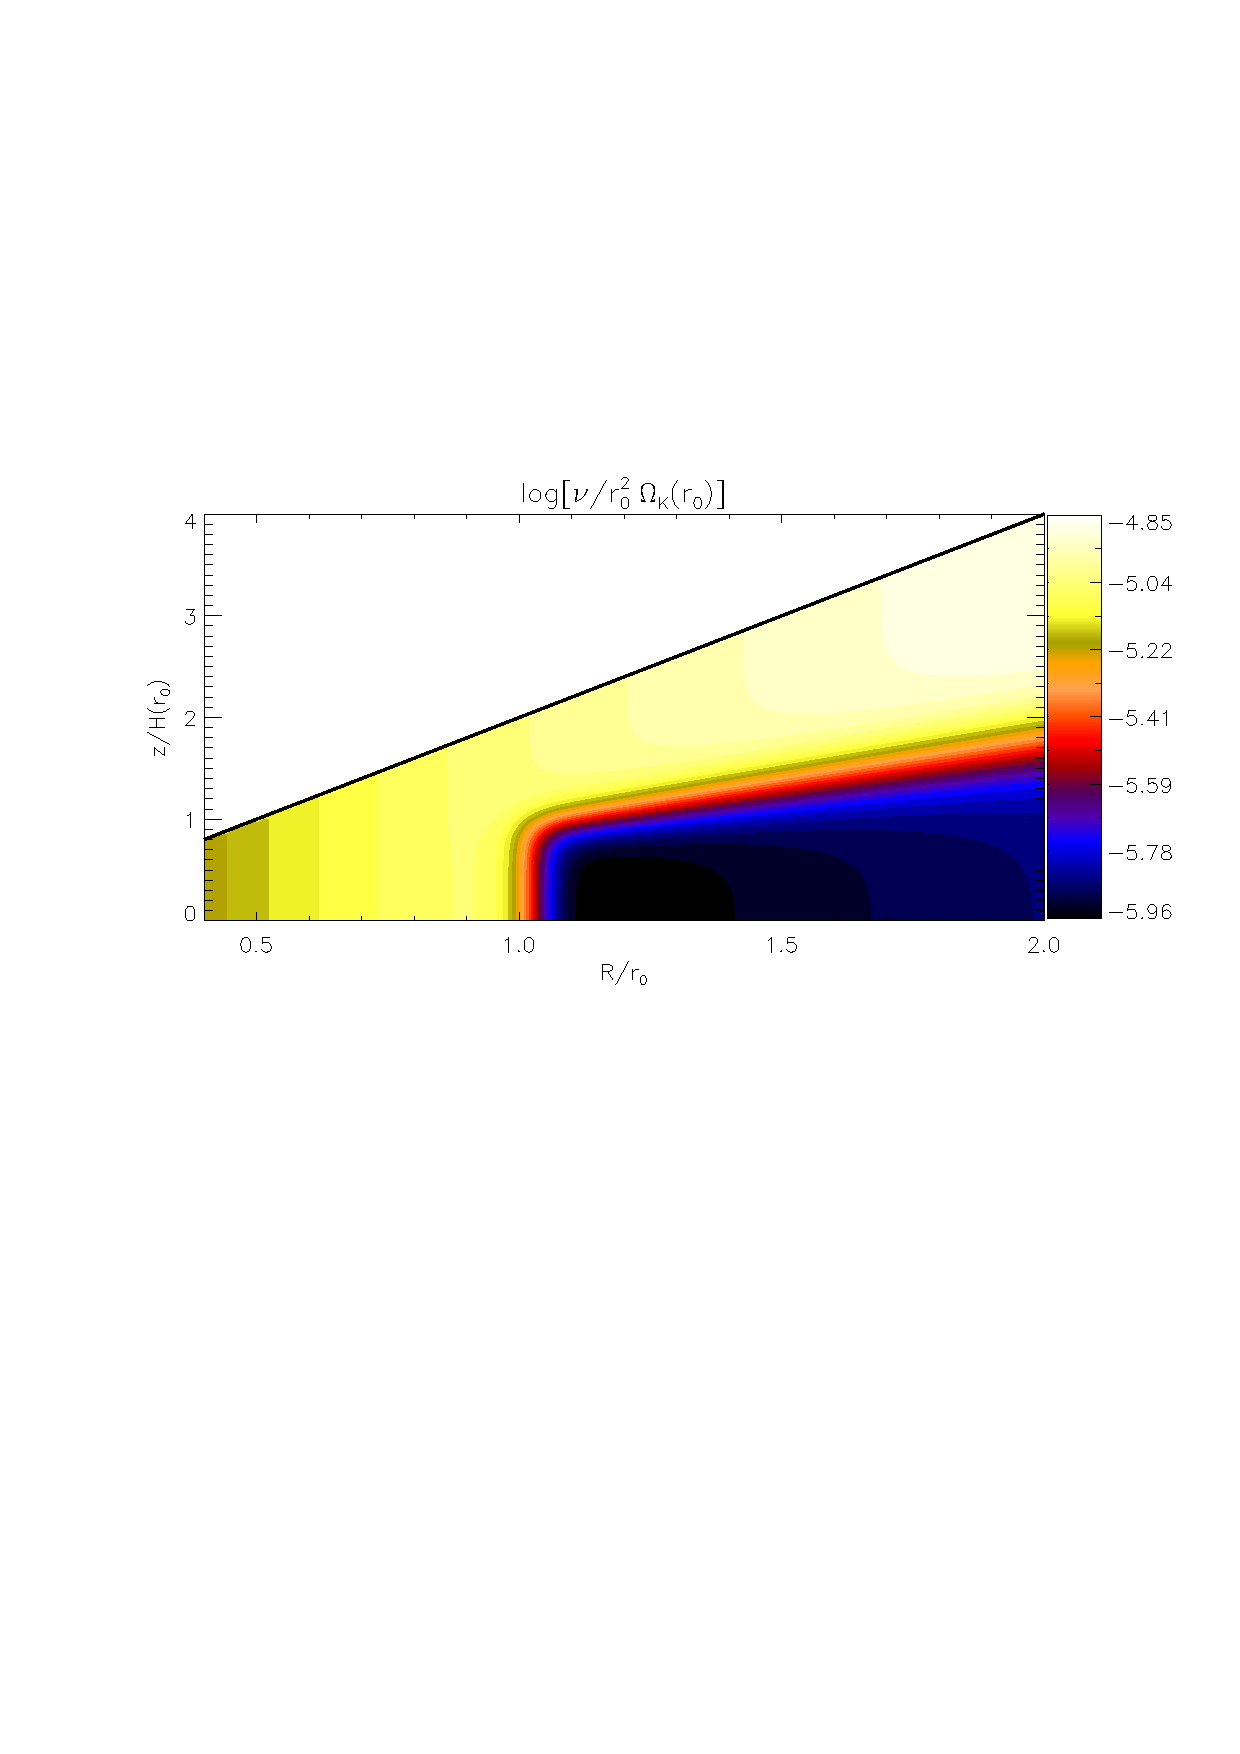
\includegraphics[width=\linewidth]{figures/pdisk_visc2d_dead}
  \caption{Example of the radially-and-vertically structured viscosity
    profile described by Eq. \ref{dead_profile}. 
    This specific plot case D2. The solid line delineates the upper
    boundary of the computational domain. 
    \label{visc2d_dead}}
\end{figure}

\subsection{Setup}
We consider discs with $h=0.1$, radial range
$[\rin,\rout]=[0.4,2.0]r_0$ and vertical size $n_h=2$. No surface
density bump is used ($A=1$). The resolution
is $(N_r,N_\theta,N_\phi)=(256,64,512)$. We initialise the disc
without radial flow, but impose perturbations to $v_r$ just after
initialisation. Note that the initial condition is not a steady-state
equilibrium solution.   

\subsection{Dead zone simulations}
Our fiducial simulation, case D0, does not have a viscous layer in the
vertical diretcion. We then consider cases D1 
and D2 with angular transitions at $\zeta_\nu=1.5h$ and
$\zeta_\nu=1.0h$, which gives a viscous layer occupying
$25\%$ and $50\%$ of the uppermost vertical domain. That is, the 
viscous layer at unit radius has thickness $0.5H_0$ and $H_0$ for
cases D1 and D2, respectively. Table \ref{dead_sims} summarises the
simulations in this section. 
 
\begin{table}
  \centering
  \caption{Summary of dead zone simulations. These runs employ the viscosity profile 
    described by Eq. \ref{dead_profile}, which invovles a viscosity
    transition both radially and vertically. The viscous layer is quoted
    as a fraction of the vertical domain at $R=r_0$. \label{dead_sims}}
  \begin{tabular}{lcccc}
    \hline\hline
    Case & $\Delta R_\nu/H_0$ & $A_\nu$ &$\zeta_\nu/h$ & visc. layer \\ 
    D0 &  0.5    &    10      &    n/a      & 0     \\%&      -0.21 \\
    D1 &  0.5     &    10     &    1.5      & $25\%$ \\% &    -0.28 \\
    D2 &  0.5     &    10     &    1.0      & $50\%$ \\%&     -0.08 \\
    \hline
  \end{tabular}
\end{table}


\subsection{Results}
To obtain an overview of disc evolution, we compare the minimum Rossby 
numbers near $R=r_0$ between cases D0, D1 and D2 in
Fig. \ref{rtrans_nuamp10_minrossby}. {\bf to be updated}.  The Rossby
number decreases when non-axisymmetric disturbances develop at
the dead zone boundary. The non-smooth evolution signifies vortex
merging. Evidently, the evolutionary timescales vary between these
cases. So we compare them at similar evolutionary stages.   

%% Cases Db0 and Db1 evolve
%% similarly, with a time-shift between them. 
%% Over the course of the simulation, both cases reach a 
%% minimum Rossby number $\sim -0.3$ at $t\simeq 120P_0,\,170P_0$ for the
%% case Db0 and Db1, respectively. We find this minima coincided with
%% vortex merging, the result being a single vortex which subsequently elongates
%% and weakens. Case Db2 evolves quite differently, it attains a minimum Rossby
%% number of $Ro\simeq-0.08$ at $t=150P_0$. This is much weaker than the
%% two previous cases, but the vortex does not weaken afterwards ($|Ro|$
%% remains roughly constant for $t\gtrsim 150P_0$).  

\begin{figure}
  \centering
  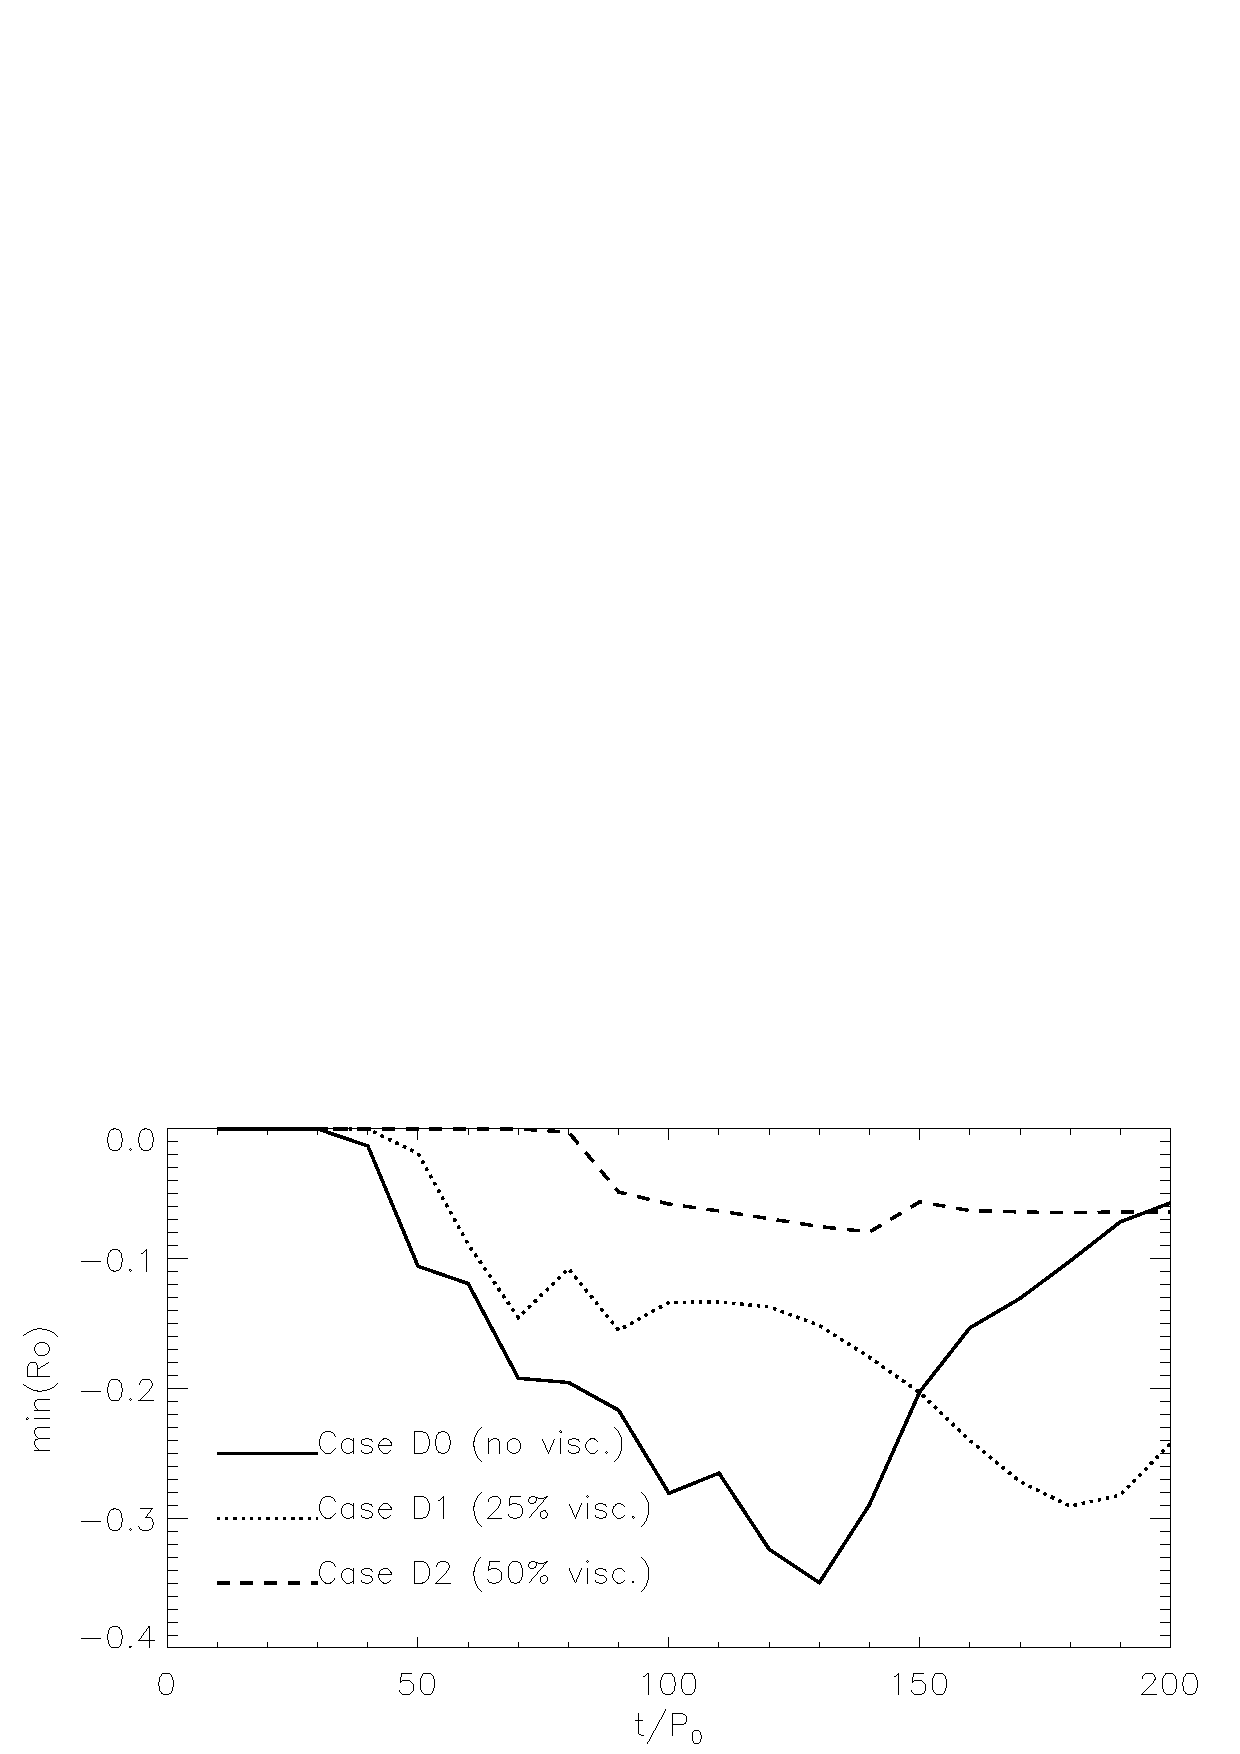
\includegraphics[width=\linewidth]{figures/rtrans_nuamp10_minrossby}
  \caption{Minimum midplane Rossby number found in case D0 (solid),
    D1, and D2 (dashed). The thickness of the viscous layer is quoted
    as the fraction of the uppermost vertical domain. 
    \label{rtrans_nuamp10_minrossby}}
\end{figure}

Fig. \ref{rtrans_nuamp10_vorten1d} shows the PV profiles as a result
of the mass build-up at the dead zone boundary. The snapshot for each
case is taken just before $Ro$ begins to decrease. 
The latter is neccessary for the RWI. We
therefore consider these profiles as the `basic state' for the
RWI. Although convenient, this is not strictly correct because the
profiles in Fig. \ref{rtrans_nuamp10_vorten1d} do not correspond to
steady states, with respect to which a linear instability is defined.   

The radial viscosity transition leads to a PV maximum and a PV minimum
on either side of unit radius. The latter is associated with the RWI. 
Case D0 and D1 have very smililar profiles, while the PV minimum is
slightly less sharp in case D2. Thus, the disc profile necessary for
instability is affected by the presence of a viscous layer. We expect
the RWI to grow more slowly in case D2 than the other cases. 

\begin{figure}
  \centering
  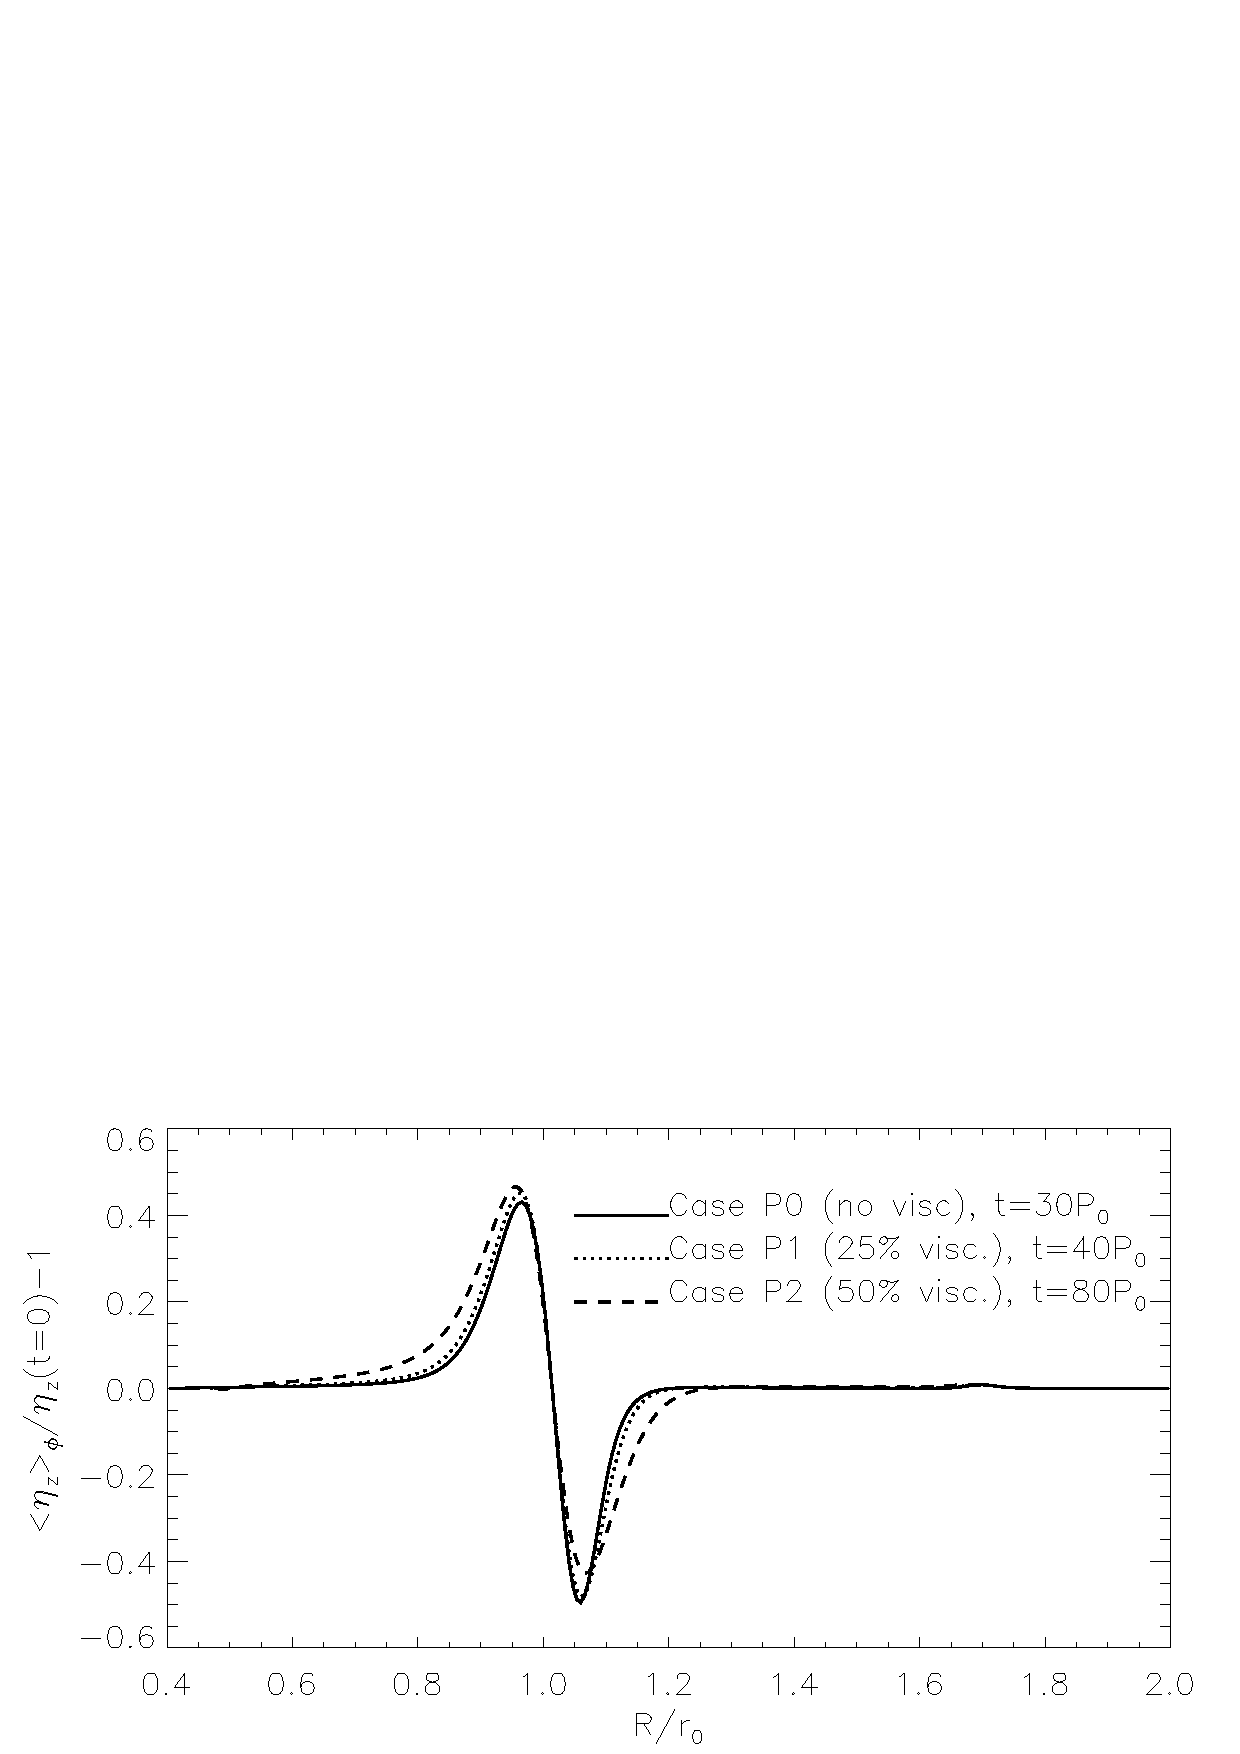
\includegraphics[width=\linewidth]{figures/rtrans_nuamp10_vorten1d}
  \caption{Potential vorticity profiles for dead zone simulations D0,
    D1 and D2. The snapshots are taken just before the Rossby numbers
    in Fig. \ref{rtrans_nuamp10_minrossby} first begins to decrease. 
    \label{rtrans_nuamp10_vorten1d}}
\end{figure}

Fig. \ref{rtrans_vdamp0_nuamp10} compares $\delta\rho$ at
$t=50P_0,\,60P_0$ and $100P_0$ for cases D0, D1 and D2, respectively.
The snapshots correspond to initial vortex formation. It is also when
the midplane $\min(Ro)$ first becomes non-negligible (see
Fig. \ref{rtrans_nuamp10_minrossby}). As expected from the PV
profiles, cases D0 and D1 are very similar, both developing the $m=3$
mode. However, case D2 develops the $m=2$ mode, because the PV extrema
is smoother. 

With the observed azimuthal wavenumbers in
Fig. \ref{rtrans_vdamp0_nuamp10}, we estimate the non-axisymmetric
mode growth rates to be $q_3\sim 0.1\Omega_0,\,0.09\Omega_0$ for cases D0 and D1; and
$q_2\sim0.05\Omega_0$ for case D2. The co-rotation radii were
%rates 0.11, 0.093 and 0.049
$r_c\sim1.073r_0,\,1.075r_0$ and $1.081r_0$, which are very close to
the radii of PV minima in Fig. \ref{rtrans_nuamp10_vorten1d}. Note
that the growth timescale is a few $P_0$, which is shorter than the
timescale to attain the PV extrema.  

\begin{figure}
   \centering
   \includegraphics[scale=.27,clip=true,trim=0cm 0.0cm 0cm
     0cm]{figures/rtrans_vdamp0_nuamp10_pdisk005.ps}\includegraphics[scale=.27,clip=true,trim=2.3cm
     0.0cm 0cm
     0cm]{figures/rtrans_vdamp2_nuamp10_pdisk006.ps}\includegraphics[scale=.27,clip=true,clip=true,trim=2.3cm
     0.0cm 0cm
     0cm]{figures/rtrans_vdamp3_nuamp10_pdisk010.ps}%% \\
    %% \includegraphics[scale=.27,clip=true,trim=0cm 1.84cm 0cm
    %%  .99cm]{figures/rtrans_vdamp0_nuamp10_vort005.ps}\includegraphics[scale=.27,clip=true,trim=2.3cm
    %%  1.84cm 0cm
    %%  0.99cm]{figures/rtrans_vdamp2_nuamp10_vort006.ps}\includegraphics[scale=.27,clip=true,clip=true,trim=2.3cm
    %%  1.84cm 0cm
    %%  0.99cm]{figures/rtrans_vdamp3_nuamp10_vort009.ps}
   \caption{Density perturbation $\delta\rho$ for dead zone simulations
     D0 (left), D1 (middle), and D2 (right). The snapshots are
     taken when $\max[\delta\rho(z=0)]$ first exceeds 0.2. 
     \label{rtrans_vdamp0_nuamp10}}
\end{figure}

%% In Fig. \ref{rtrans_vdamp0_nuamp10_2} we compare the final vortex just after its formation
%% (when $Ro$ reaches its minimum with respect to time). 
%% Cases Db0 and Db1 are again similar, developing a compact vortex with $Ro \sim -0.3$. However,
%% we found that this vortex weakens thereafter. On the other hand case Db2 , despite forming
%% a weaker vortex ($Ro\sim -0.07$).

The minimum midplane Rossby number attained is
$\min[Ro(z=0)]=-0.35,\,-0.29,\,-0.08$ for cases D0, D1 and D2,
respectively. The corresponding density perturbation is shown in
Fig. \ref{rtrans_vdamp0_nuamp10_2}. The vortex in case D1 is only slightly
weaker and larger than D0. However, snapshot for D1 is taken about
$50P_0$ later than D0. This, together with the above results,
indicates that introducing a relatively small viscous layer (recall
case D1 has a viscous layer of thickness $0.5H_0$) mainly shifts the
time evolution. In other words, the timescale required for vortex
formation is lenghtened by introducing the viscous layer, but the
characteristics of the final vortex is not much affected. 

Case D2, on the other hand, evolves differently. It only attains
$\min[Ro(z=0)]= -0.08$ so the vortices are noticeably weaker than
cases D0/D1, as is the density flucuation $\delta\rho$. As shown
in Fig. \ref{rtrans_vdamp0_nuamp10_2}, the vortex in case D2 is much
more elongated than previous runs. This is somewhat surprising because
the basic states are not significantly different (with similar growth
rates). 
%% Also in case D2 $Ro$ remains roughly
%% constant after reaching its minimal value, while in cases D0/D1
%% the vortex becomes weaker toward the end of the runs. 
%Also consistent with previous simulations, vortex-merging
%is resisted. 

\begin{figure}
   \centering
   \includegraphics[scale=.27,clip=true,trim=0cm 0.91cm 0cm
     0cm]{figures/rtrans_vdamp0_nuamp10_pdisk013.ps}\includegraphics[scale=.27,clip=true,trim=2.3cm
     .91cm 0cm
     0cm]{figures/rtrans_vdamp2_nuamp10_pdisk018.ps}\includegraphics[scale=.27,clip=true,clip=true,trim=2.3cm
     .91cm 0cm
     0cm]{figures/rtrans_vdamp3_nuamp10_pdisk014.ps}\\
    \includegraphics[scale=.27,clip=true,trim=0cm 0.cm 0cm
      .99cm]{figures/rtrans_vdamp0_nuamp10_vort013.ps}\includegraphics[scale=.27,clip=true,trim=2.3cm
      0.0cm 0cm
      0.99cm]{figures/rtrans_vdamp2_nuamp10_vort018.ps}\includegraphics[scale=.27,clip=true,clip=true,trim=2.3cm
      0.0cm 0cm
      0.99cm]{figures/rtrans_vdamp3_nuamp10_vort014.ps}
    \caption{Density perturbation $\delta\rho$ (top) and
      Rossby number $Ro$ (bottom) for cases D0 (left), D1
      (middle), and D2 (right). Snapshots are taken when
      $\mathrm{min}[Ro(z=0)]$ is attained. 
      \label{rtrans_vdamp0_nuamp10_2}}
\end{figure}

